\subsection{\ours Overview}
\label{sec:overview}

\begin{figure*}[t]
    \centering
    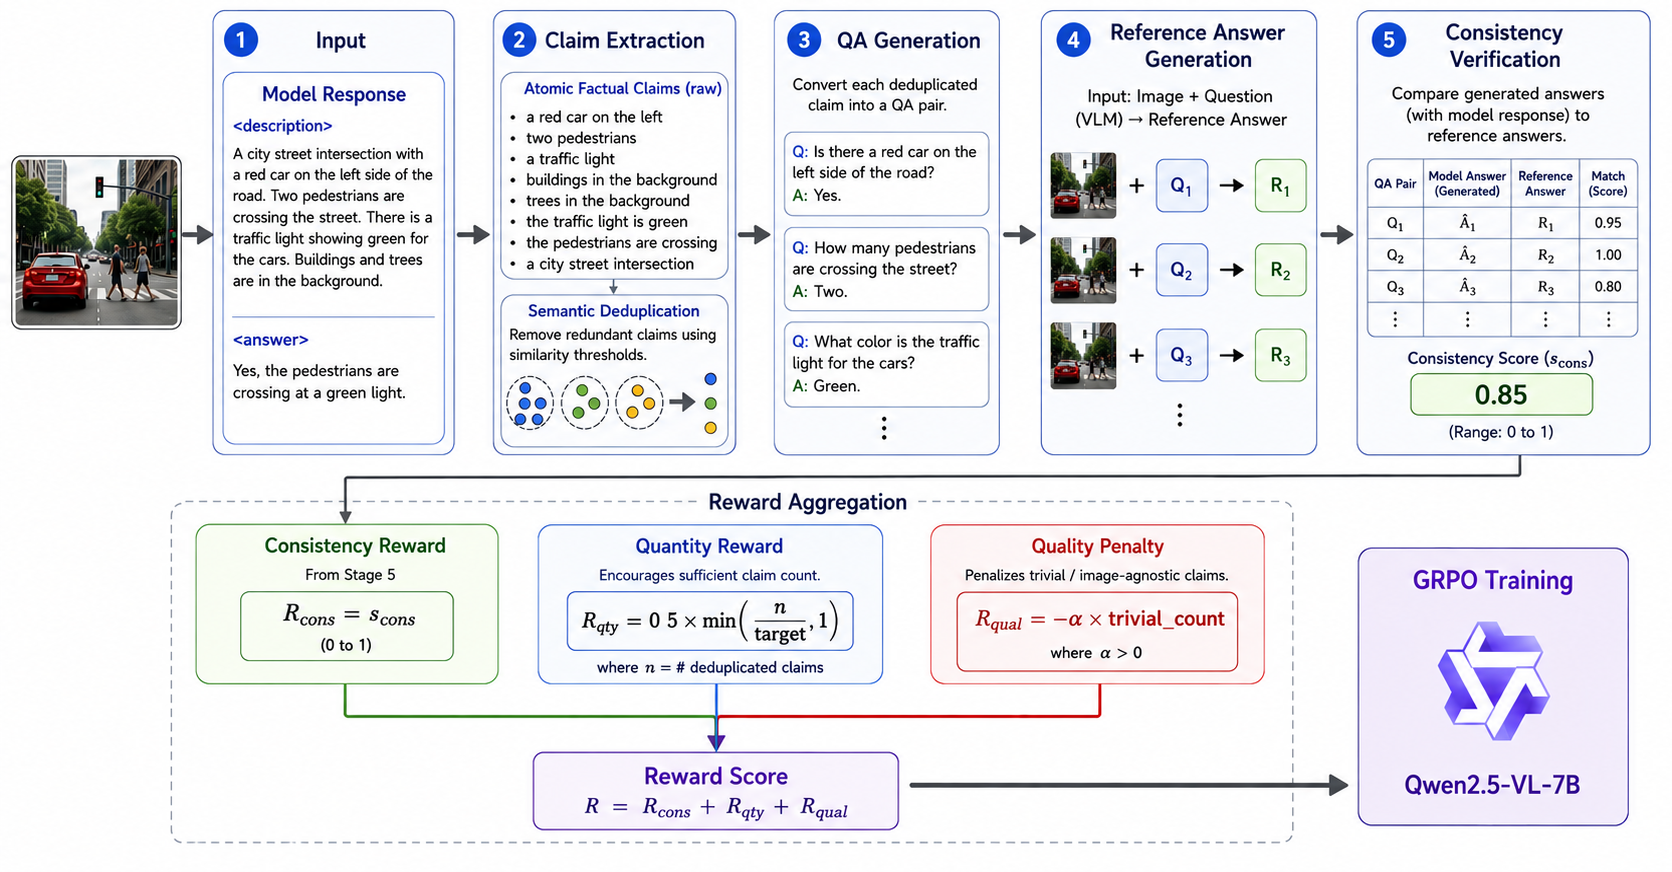
\includegraphics[width=\textwidth]{figures/pipeline.png}
    \caption{Overview of the \ours pipeline. Given a model-generated response,
    \ours first extracts atomic factual claims from the generated description
    and removes semantically redundant claims. Each remaining claim is converted
    into a visual question-answer pair, where the answer is implied by the
    generated description. The VLM then answers the same questions using the
    original image, producing image-grounded reference answers. The consistency
    between the implied answers and the reference answers is verified through
    majority voting. In addition, Visual Evidence Calibration (VEC) calibrates
    the reward by encouraging diverse claims, rewarding sufficient claim
    coverage, and penalizing claims answerable from degraded visual evidence.}
    \label{fig:pipeline}
\end{figure*}

\ours converts open-ended visual factuality evaluation into a set of fine-grained answer consistency checks. Given a generated response, \ours decomposes it into atomic claims, transforms each claim into a visual question-answer (QA) pair, obtains an image-grounded reference answer, and verifies consistency between the two. This \emph{asymmetric} design decouples generation from verification: the reference answer is derived solely from the image, not from the original response, mitigating the self-confirmation bias inherent in single-model verification.

Formally, the self-verifying reward is
\begin{equation}
    R_{\mathrm{SV}}(I,q,y) = R_{\mathrm{cons}} + R_{\mathrm{VEC}},
\end{equation}
where $R_{\mathrm{cons}}$ is a claim-level consistency score and $R_{\mathrm{VEC}}$ is the Visual Evidence Calibration term, described below.

\subsection{Claim-Level Self-Verification}
\label{sec:claim_level_verification}

\paragraph{Claim Extraction.}
Given description $y^{\mathrm{desc}}$, \ours extracts a set of atomic factual claims:
\begin{equation}
    \mathcal{C} = \{c_1,\ldots,c_m\} = \mathrm{Extract}(y^{\mathrm{desc}}).
\end{equation}
Each $c_i$ is a short, self-contained statement about a single visual fact (e.g., object existence, color, quantity, spatial relation), enabling fine-grained verification rather than coarse response-level judgment.

\paragraph{Semantic Deduplication.}
Raw claims may be repeated or semantically overlapping, which can be exploited for reward hacking. We therefore deduplicate using cosine similarity between sentence embeddings $\phi(\cdot)$:
\begin{equation}
    \mathrm{sim}(c_i,c_j) = \frac{\phi(c_i)^\top \phi(c_j)}{\|\phi(c_i)\|\cdot\|\phi(c_j)\|}.
\end{equation}
Pairs exceeding a type-aware threshold are merged, retaining one representative. Same-type claims are deduplicated more aggressively than cross-type ones. The resulting set is $\mathcal{C}^{\ast} = \{c_1^{\ast},\ldots,c_n^{\ast}\}$, $n \leq m$.

\paragraph{Question-Answer Generation and Reference Answers.}
Each deduplicated claim $c_i^{\ast}$ is converted into a visual QA pair $(v_i, a_i) = \mathrm{QA}(c_i^{\ast})$, where $v_i$ is the question and $a_i$ is the answer implied by the claim. A reference answer is then obtained by querying the VLM on the original image:
\begin{equation}
    a_i^{\prime} = \mathrm{Ans}(I, v_i).
\end{equation}
The separation between $a_i$ (from description) and $a_i^{\prime}$ (from image) is central to the asymmetric design.

\paragraph{Answer Consistency Verification.}
A verifier $f_{\mathrm{ver}}$ compares the two answers, with robustness ensured by majority voting over $K$ runs:
\begin{equation}
    z_i = \mathbbm{1}\!\left[\sum_{k=1}^{K} z_i^{(k)} > \tfrac{K}{2}\right], \quad z_i^{(k)} = f_{\mathrm{ver}}(a_i, a_i^{\prime}).
\end{equation}
The consistency reward is the fraction of verified claims:
\begin{equation}
    R_{\mathrm{cons}} = \frac{1}{n}\sum_{i=1}^{n} z_i.
\end{equation}

\subsection{Visual Evidence Calibration}
\label{sec:vec}

Claim-level verification alone can still be exploited: the model may produce redundant claims, too few claims, or trivially easy claims answerable without genuine visual attention. VEC addresses these failure modes via three complementary mechanisms.

\paragraph{Redundancy Control.}
Semantic deduplication (described above) ensures each distinct fact is counted only once in $R_{\mathrm{cons}}$, preventing reward inflation from repetitive claims.

\paragraph{Informativeness Reward.}
To discourage under-informative responses, we add a claim-count reward capped at a target $n_{\mathrm{target}}$:
\begin{equation}
    R_{\mathrm{cnt}} = \lambda_{\mathrm{cnt}} \cdot \min\!\left(\frac{n}{n_{\mathrm{target}}}, 1\right),
\end{equation}
with $\lambda_{\mathrm{cnt}} = 0.5$, keeping factual consistency as the dominant signal.

\paragraph{Visual-Dependence Penalty.}
Some claims (e.g., ``there are objects in the image'') can be answered correctly from language priors alone. To detect such image-agnostic claims, we construct a degraded image $\tilde{I}$ (heavy Gaussian blur + grayscale + horizontal flip) and obtain $\tilde{a}_i = \mathrm{Ans}(\tilde{I}, v_i)$. A claim is marked trivial if the degraded answer matches the original reference:
\begin{equation}
    t_i = \mathbbm{1}\!\left[f_{\mathrm{ver}}(\tilde{a}_i, a_i^{\prime}) = 1 \right].
\end{equation}
% \begin{equation}
%     t_i = \mathbbm{1}\!\left[f_{\mathrm{ver}}(\tilde{a}_i, a_i^{\prime}) = 1 \;\land\; a_i^{\prime} \neq \texttt{unknown} \;\land\; \tilde{a}_i \neq \texttt{unknown}\right].
% \end{equation}
The quality penalty discourages such claims:
\begin{equation}
    R_{\mathrm{qual}} = -\lambda_{\mathrm{qual}} \sum_{i=1}^{n} t_i.
\end{equation}

The overall VEC term is $R_{\mathrm{VEC}} = R_{\mathrm{cnt}} + R_{\mathrm{qual}}$, and the final GRPO reward is:
\begin{equation}
    R_{\mathrm{SV}}(I,q,y) = R_{\mathrm{cons}} + R_{\mathrm{cnt}} + R_{\mathrm{qual}}.
\end{equation}
The three components are complementary: $R_{\mathrm{cons}}$ enforces factual grounding; $R_{\mathrm{cnt}}$ promotes coverage; and $R_{\mathrm{qual}}$ penalizes image-agnostic claims. Together, they provide a scalable, annotation-free reward for hallucination mitigation.
